\vsssub
\subsubsection{重启动文件处理器} \label{sec:ww3uprstr}
\vsssub

\proddefH{ww3\_uprstr}{ww3uprstr}{ww3\_uprstr.ftn}
\proddeff{输入}{ww3\_uprstr.inp}{传统配置文件。}{10} (App.~\ref{sec:config221})
\proddefa{mod\_def.ww3}{模式定义文件。}{20}
\proddefa{restart.ww3}{重启动文件。}{ }
\proddefa{XXXX.grbtxt}{grbtxt 格式的有效波高分析文件。}{123}
\proddeff{输出}{restart001.ww3}{更新后的重启动文件。}{ }

\vspace{\baselineskip}

\paragraph{引言 \newline}

海面波浪场的大多数观测都是诊断变量有效波高（SWH）的观测。因此，波浪资料同化（WDA）常常在 SWH 空间中进行，随后需要把这些信息转换到预报变量空间，也就是波谱（WS），以便作为边界和/或初始条件（BIC）施加。

\subparagraph{\textbf{ww3\_uprstr} 的目的 \newline}
将 SWH 场分析中的能量重新分配到保存在重启动文件中的 WS 场。

\subparagraph{核心算法 \newline}
\textbf{ww3\_uprstr} 将背景谱的 SWH 设置为等于分析 SWH，并根据用户指定的谱形修改谱的形状。\textbf{ww3\_uprstr} 作为重启动读取器的扩展实现；它需要的输入包括重启动文件、分析 SWH，以及包含用户定义选项的 \textbf{ww3\_uprstr.inp}（见上文）。为减少即时计算，可能还需要额外文件。

\paragraph{如何使用 ww3\_uprstr \newline}
使用 \textbf{ww3\_uprstr} 时，用户需要遵循与所有 WAVEWATCH III 程序相同的逻辑。概括如下：

\begin{enumerate}
   \item \textbf{下载源代码} \newline
   从 6.07 版开始，\textbf{ww3\_uprstr} 源代码已经包含在 WAVEWATCH III 官方发布版中。
   \item \textbf{编译代码} \newline
   \textbf{ww3\_uprstr} 的编译方式与 WAVEWATCH III 的其他辅助程序相同，见手册中的相应章节。若需要调试输出，在 switch 文件中使用 \textbf{T} 标志。
   \item \textbf{测试可执行程序} \newline
   回归测试 \textbf{ww3\_ta1} 可用于测试 \textbf{ww3\_uprstr} 的不同选项。
   \item \textbf{运行 ww3\_uprstr} \newline
   运行 \textbf{ww3\_uprstr} 的步骤说明：
   \begin {description}
      \item{必需输入文件：\newline}
      \begin{itemize}
         \item \textbf{重启动文件。} 该文件由 WW3 在模式后报运行或前一循环中创建。预期文件名为 \textbf{restart.ww3}。
         \item \textbf{mod\_def.ww3}
         \item \textbf{ww3\_uprstr.inp。} 这是 \textbf{ww3\_uprstr} 的输入文件。用户必须定义：i. 同化日期；ii. 能量重新分配方法；iii. 取决于所选方法的百分比或输入文件。
         \item \textbf{分析输入文件。} 文件可以使用任意名称，但后缀决定用于导入数据的读取器。对大多数选项，读取器仅支持 \textbf{grbtxt} 格式。这是一个由 wgrib2 从分析 grib2 文件创建的文本文件，其结构如下：\newline

         \begin{tabular}{|c|}
            \hline
            NX NY       \\
            VAL0001     \\
            VAL0002     \\
            ...         \\
            VAL(NX*NY)  \\
            \hline
          \end{tabular}
    \newline
    \item 运行可执行程序：\newline
          \textgreater \$EXE/ww3\_uprstr \newline
          如果所有输入都准备正确，将创建新的重启动文件（\textbf{restart001.ww3}）。\textbf{ww3\_uprstr} 按与 restart.ww3 相同的格式导出更新后的谱。若要把它作为下一预报循环初始化的 BIC 使用，必须将其改名：\newline
          \textgreater mv \textbf{restart001.ww3} \textbf{restart.ww3}) \newline
          更新后的重启动文件随后即可按常规方式使用。
      \end{itemize}
   \end{description}

   \noindent\fbox{
      \parbox{\textwidth}{
         \textbf{提示}
         \begin{itemize}
            \item 重启动文件必须使用与 \textbf{ww3\_uprstr} 相同的 WW3 版本创建；该工具不提供向后兼容性。
            \item 在 \textbf{ww3\_uprstr.inp} 中定义的同化开始时间必须与重启动文件中的时间一致。
            \item 使用 \textbf{T} 时，\textbf{ww3\_uprstr.inp} 会导出背景重启动文件、分析以及更新后重启动文件中的 SWH 场。此外，更新前后的重启动文件谱也会作为文本文件导出。
         \end{itemize}
         }
   }
\end{enumerate}

\subparagraph{更新方法 \newline}
用户必须在 \textbf{ww3\_uprstr.inp} 中定义自己选择的更新算法。更新重启动文件的选项通过标志 UPD[N] 在 ww3\_uprstr.inp 中定义，其中 N 可以为 0F、0C、1、2 等。对于 N \textless 2 的 UPDN，同一修正应用于整个网格；预期输入为 PRCNTG，如 fac 所定义。对于 N \textgreater 1 的 UPDN，每个网格点都有自己的更新因子，输入为 grb2txt 格式。当前实现的更多细节见图~\ref{fig:uprstrflowchart}。

\begin{figure} \begin{center}
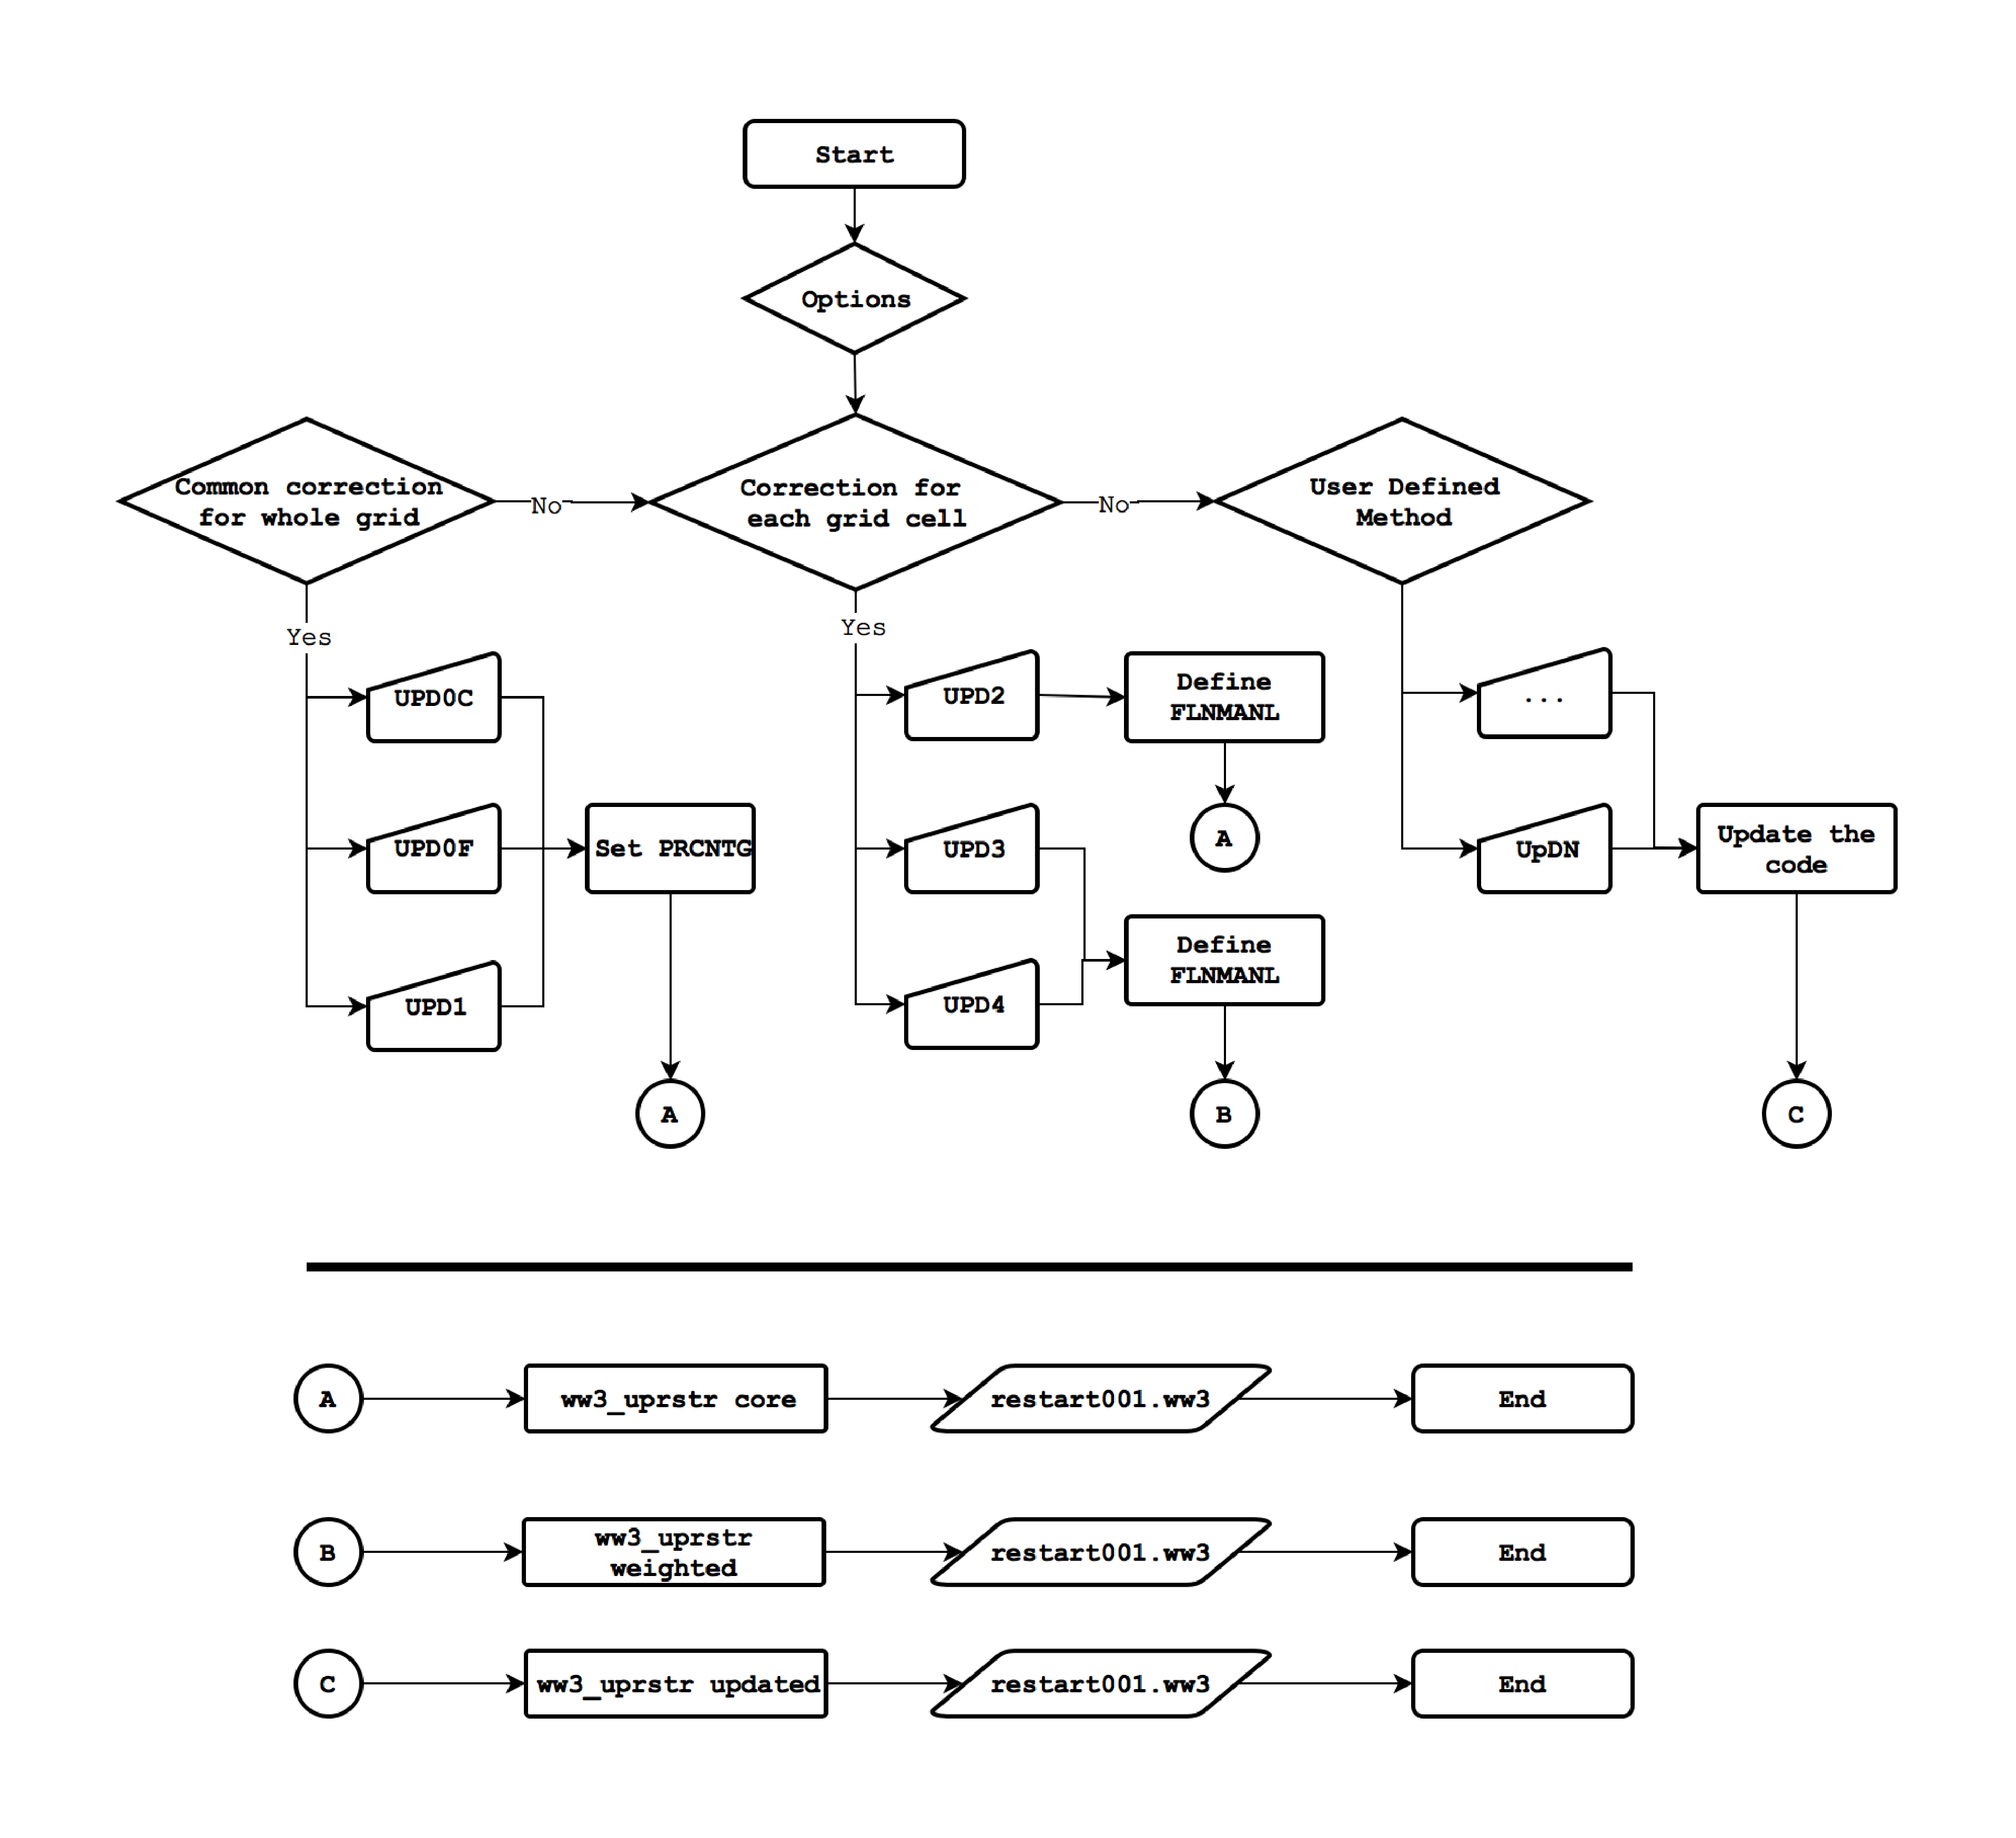
\includegraphics[width=0.9\textwidth]{./run/uprstr.eps}
\caption{WW3 重启动文件中波谱更新方法的实现流程图。可通过在 namelist 中增加 UPD 选项来实现其他方法。}
\label{fig:uprstrflowchart} \botline
\end{center}
\end{figure}

目前可用的 UPD 选项如下：
\begin{enumerate}
   \item UPD0C:: \textbf{自 5.16 版起已删除} 选项 0C，所有谱使用一个常数更新：\newline
      \(fac=(SWH\_Bckg-SWH\_Anl)/SWH\_Anl \).
   \item UPD0F:: 选项 0F，所有谱使用一个常数更新：\newline
      \(fac=SWH\_Anl/SWH\_Bckg \).
   \item UPD1 :: \textbf{自 5.16 版起已删除} 选项 1，fac(x,y,frq,theta) 按每个谱箱中的能量百分比加权；fac 与 UPDOF 相同。
   \item UPD2 :: 选项 2，根据 SWH\_Bckg 和 SWH\_Anl 在每个网格点计算 fac(x,y,frq,theta)。
   \item UPD3 :: 选项 3，更新因子是一个具有背景谱形状的曲面。
   \item UPD4 :: [当前版本未包含，仅保留位置] 选项 4，UPD3 的一般化。更新因子为多个曲面的和，这些曲面施加到背景谱上。该算法需要将每个分区映射到单个谱；该映射用于确定加权曲面。
   \item UPD5 :: 选项 5，修正按 UPD2 计算，但仅当风海为主导分量时才应用于谱的风海部分；否则修正整个谱。必需输入为分析 Hs 场，以及背景风速和风向。若要包含风数据，建议运行使用 WRST 开关构建的代码。
   \item UPD6 :: 选项 6，修正按 UPD5 计算，但风海分量还会使用 Toba (1973) 在频率空间中移动。必需输入为分析 Hs 场，以及背景风速和风向。若要包含风数据，建议运行使用 WRST 开关构建的代码。
\end{enumerate}

可以通过进一步扩展输入文件并向 \textbf{ww3\_uprstr.ftn} 添加源代码，加入其他用于将能量重新分配到 WS 并修正相关风场的方法。

\subparagraph{示例 \newline}
本节讨论一个最简单 WDA 应用的示例。图~\ref{fig:waveDAflowchart} 展示了 \textbf{ww3\_uprstr} 如何在一个简单波浪分析系统框架中使用。\newline

一次 WW3 运行（来自前一循环或来自后报）在适当时间提供 SWH 背景场以及对应的重启动文件。背景 SWH 场的格式必须与 WDA 模块输入兼容。

\begin{figure} \begin{center}
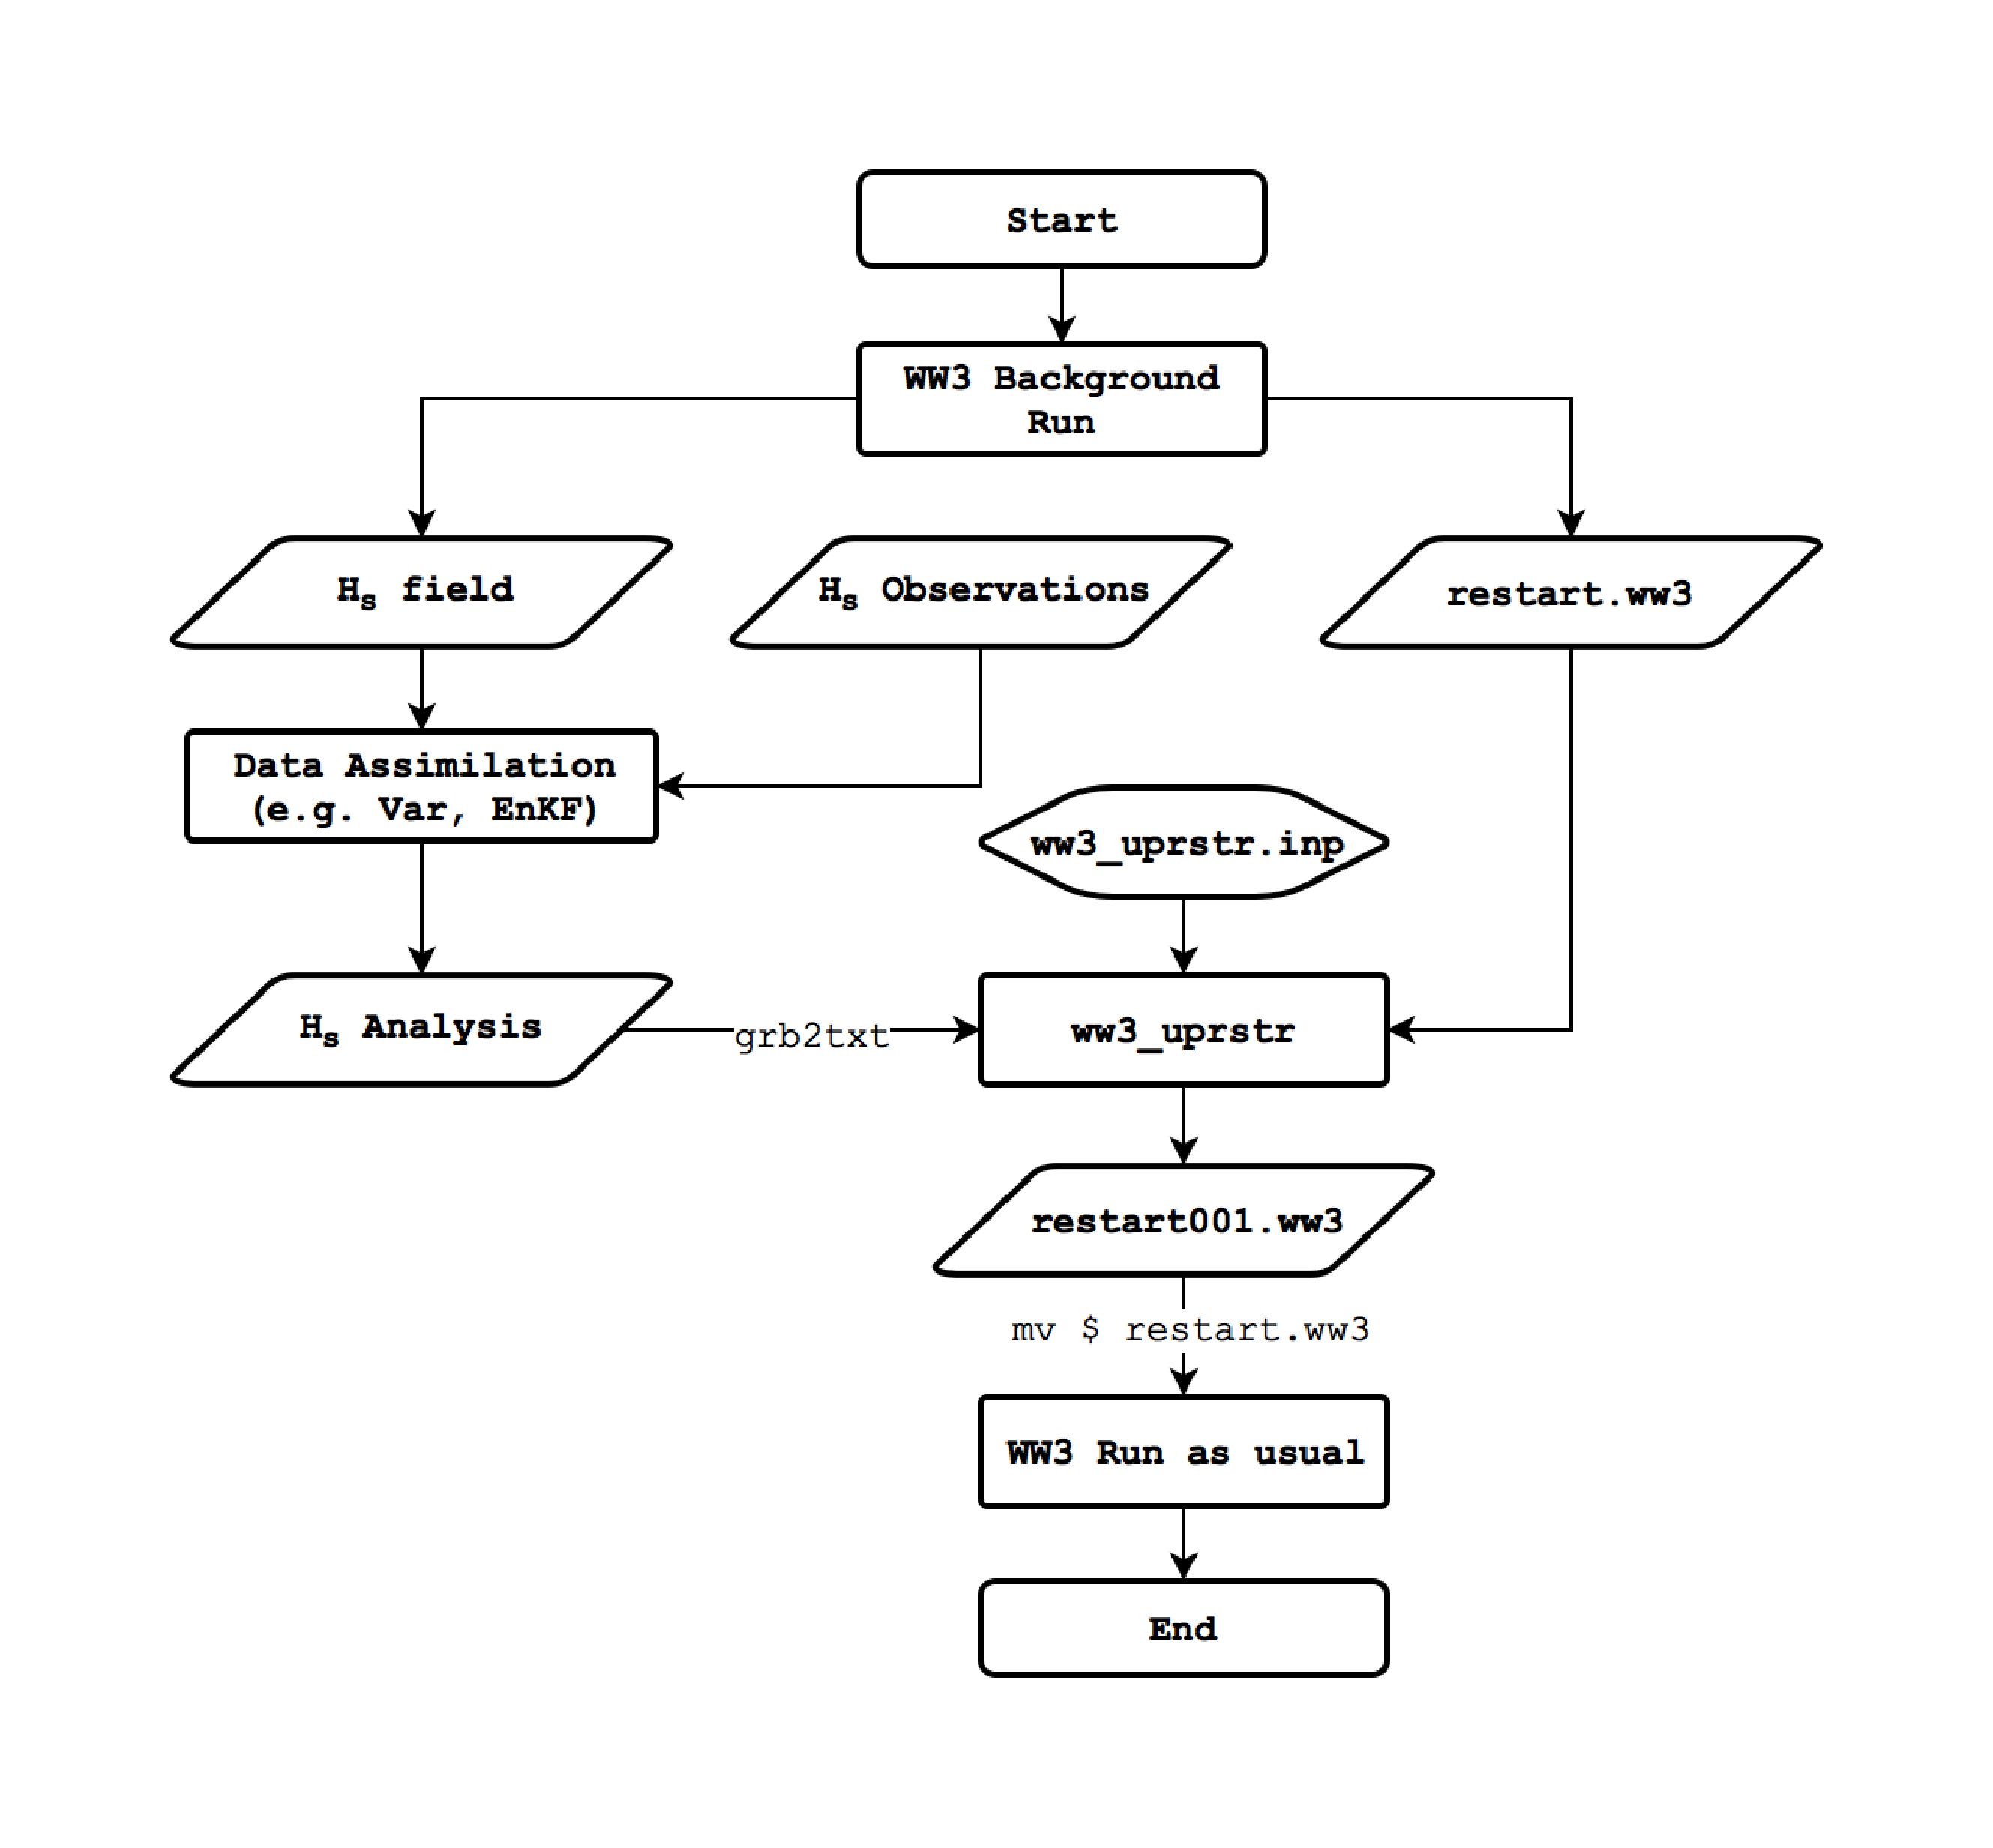
\includegraphics[width=0.9\textwidth]{./run/waveDA.eps}
\caption{简化波浪资料同化系统的流程图，展示 {ww3\_uprstr} 的作用、所需输入文件以及更新后重启动文件的输出结果。}
\label{fig:waveDAflowchart} \botline
\end{center}
\end{figure}

WDA 模块使用背景场和分析时刻可用的观测，生成分析，并以 grbtxt 格式（\textbf{XXXX.grbtxt}）导出 SWH 场。

分析文件、\textbf{mod\_def.ww3}、\textbf{restart.ww3} 文件以及 \textbf{ww3\_uprstr.inp} 是 \textbf{ww3\_uprstr} 的输入文件。如果所有选项和输入文件都准备正确，在单处理器上更新包含 260000 个网格节点的网格并生成输出大约需要一分钟。更新后的重启动文件必须改名为预期文件名；在本例中为 \textbf{restart.ww3}。\newline

   \noindent\fbox{
      \parbox{\textwidth}{
      \textbf{注意：}
      所有 \ncep{} 的 WDA 系统都使用 GRIB2 格式，因此总是需要一个中间步骤将 grib 文件转换为合适格式。所用软件为 WGRIB2，更多信息可从
      \href{http://www.cpc.ncep.noaa.gov/products/wesley/wgrib2}{官方网站} 获取。
      }
   }

%\paragraph{如何更新 ww3\_uprstr \newline}
%添加数据读取器，主要用于机器无关二进制数据和 wgrib2。

\pb
